% SPDX-License-Identifier: LPPL-1.3c
% Copyright (C) 2026 Christophe Jorssen
% Author and Current Maintainer: Christophe Jorssen <christophe.jorssen@gmail.com>
% LPPL maintenance status: maintained
% This file is part of luafemm. See LICENSE and LICENSES.md for its terms.
\section{Axisymmetric magnets and circular windings}
\label{sec:axisymmetric}

\subsection{A rectangle that becomes a solenoid}
A finite solenoid is naturally described in a meridional section.
A planar drawing of two opposite current rectangles would describe a device
invariant along the direction out of the page. The coil is a body of
revolution. Draw only its meridional half-section: the horizontal
coordinate is the radius $r\geq0$, and the vertical coordinate is $z$.
Rotating one copper rectangle about the vertical axis produces the whole
winding volume. There is no second return rectangle at negative radius.

Start with a reusable style. It selects the geometry before setting its
bounds, so the meaning of every subsequent coordinate is clear.
\begin{codeexample}[code only]
\tikzset{solenoid/.style={
  femm/problem={type=axisymmetric,
    xmax=100,ymin=-85,ymax=85,mesh size=4},
  femm/circuit={name=coil,current=2}}}
\end{codeexample}
The coordinate unit is still one millimetre in the TikZ interface. The axis is
$r=0$, and |type=axisymmetric| sets |xmin=0|. The regularity condition there is
automatic. Other exterior sides default to zero azimuthal vector potential;
they are a finite truncation of the surrounding air, not an exact infinite
boundary. Enlarge the air domain separately from refining the mesh.

A single region now declares 300 circular turns carrying 2 A:
\begin{codeexample}[code only]
\filldraw[fill=orange!25,draw=orange!70!black,
  femm/region={material=copper,circuit=coil,turns=300,
    winding fill=.6,mesh size=1}]
  (20,-30) rectangle (30,30);
\end{codeexample}
Positive current flows along $+\varphi$ and gives a positive axial field in the
bore. The current density is $NI/S$, with $S$ the active meridional winding
area. The fill factor changes the electrical resistance; it does not reduce
these declared ampere-turns. Signed turns reverse the excitation.

Before solving, register a profile on the axis. The existing drawing
and plotting commands keep their usual TikZ/PGFPlots syntax:
\begin{codeexample}[code only]
\path[femm/profile={name=solenoid-axis,samples=121}]
  (0,-60)--(0,60);
\pic[femm/lines=17] {femm field};
% In an ordinary PGFPlots axis:
\femmplot[profile=solenoid-axis,component=Bz,abscissa=z]
\end{codeexample}
The lines represent contours of the full flux $\Phi=2\pi rA_\varphi$.
Contours of $A_\varphi$ alone would not be magnetic field lines. Arrows follow
$(B_r,B_z)$, and equally spaced flux levels enclose equal full-revolution flux.
The profile samples the unsmoothed finite-element field, including its jumps
between elements. Increasing |samples| draws those jumps more densely; it does
not refine the field solution.

The example additionally refines the bore and compares its axial
profile with the Biot--Savart integral for the same uniformly filled coil in
infinite air. It also reports the winding resistance and secant inductance.
\luafemmexamplebegin{axisymmetric-solenoid}

Define the solenoid once, then use its saved axial profile in a separate axis. The coil rectangle represents all the circular turns.

% manual example: axisymmetric-solenoid/1

\begin{codeexample}[setup code]
\tikzset{solenoid/.style={femm/problem={type=axisymmetric,
    xmax=100,ymin=-85,ymax=85,mesh size=4,contour subdivisions=2},
    femm/circuit={name=coil,current=2}},
  coil section/.style={draw=orange!70!black,fill=orange!25,
    femm/region={material=copper,circuit=coil,turns=300,
      winding fill=.6,mesh size=1}}}
\end{codeexample}

The following picture uses the preceding definitions.

% manual example: axisymmetric-solenoid/2

\begin{codeexample}[width=0pt]
\begin{tikzpicture}[solenoid,scale=.55,
    femm/cache={file=\jobname,mode=auto}]
  \path[femm/region={material=air,mesh size=1}] (0,-65) rectangle (35,65);

  \filldraw[coil section] (20,-30) rectangle (30,30);
  \pic[femm/lines=17,femm/arrow spacing=18mm] {femm field};
  \draw[dashed,gray] (0,-85)--(0,85) node[above] {$z$};
  \draw[red,dashed,femm/profile={name=solenoid-axis,samples=121}]
    (0,-60)--(0,60);
  \draw[-Stealth] (0,-90)--(40,-90) node[right] {$r$};
  \node[fill=orange!25] at (25,0) {$\odot$};
  \femmmeasure[name=solenoid-coil,quantity=circuit,circuit=coil]
\end{tikzpicture}
\end{codeexample}

% manual example: axisymmetric-solenoid/3

\begin{codeexample}[width=0pt]
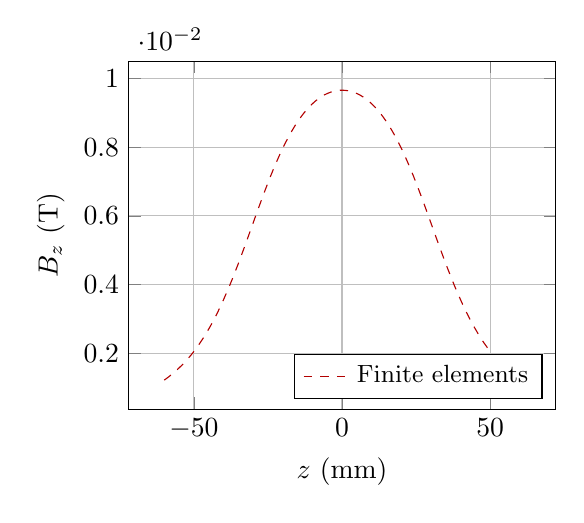
\begin{tikzpicture}
\begin{axis}[width=7cm,height=6cm,grid=major,no markers,
    xlabel={$z$ (mm)},ylabel={$B_z$ (T)},legend style={font=\small},
    legend pos=south east]
  \femmplot[profile=solenoid-axis,component=Bz,abscissa=z,
    plot options={blue!65!black,thick}]
  \addlegendentry{Finite elements}

  \addplot[red!70!black,dashed,domain=-60:60,samples=121]
    {0.000628318530718*((30-x)*ln((30+sqrt(900+(30-x)^2))/
      (20+sqrt(400+(30-x)^2)))+(30+x)*ln((30+sqrt(900+(30+x)^2))/
      (20+sqrt(400+(30+x)^2))))};
  \addlegendentry{Infinite-air reference}
\end{axis}
\end{tikzpicture}
\end{codeexample}

\luafemmexampleend{axisymmetric-solenoid}

Start with coarse global spacing and local refinement where the field is
observed. Once the drawing and excitation are settled, reduce both spacings,
then move the outer boundary. The analytic reference has no artificial outer
boundary, whereas the finite-element example does. A small discrepancy can
therefore contain both mesh and exterior-truncation error. Drawing more flux
lines or subdividing their display mesh changes neither error.

\subsection{Choosing the problem and rendering the flux}
\begin{key}{/femm/problem/type=\meta{choice} (initially planar)}
A PGF choice handler selecting |planar|, |axisymmetric| or |axial|.
The first two are vector-potential models; the transverse |axial| model is
described in Section~\ref{sec:currents}. All retain ordinary paths, compound
regions, material styles and the generic TeX loaders.
The axisymmetric choice sets |xmin=0|; place |type| before an explicit positive
|xmin| when modelling a domain that does not touch the axis. Returning to
|planar| does not reset bounds that have already been chosen.

For axisymmetry, all coordinates must have nonnegative radius. Every connected
component must touch the axis or have a Dirichlet or positive Robin anchor.
The solver rejects unanchored annular components rather than imposing
an arbitrary planar potential gauge. |depth| has no physical effect: the
problem represents a complete revolution, not a slice of prescribed thickness.
Imported FEM files select their own problem type; an explicit conflicting
|type| is rejected. Declaring only |type=axisymmetric| while importing does not
override bounds supplied by the file.
\end{key}

\begin{key}{/femm/problem/contour subdivisions=\meta{integer} (initially 2)}
For axisymmetric field rendering, subdivide every drawing triangle into four
at each level, from 0 to 4. The default therefore uses 16 drawing triangles
per solution element. The quadratic flux $2\pi rA_\varphi$ is evaluated at the
subdivision vertices and traced by the existing stitched marching-triangle
renderer. This is a controlled drawing approximation; it creates no solver
nodes, changes no measured field and does not invalidate a cached solution.
Large values increase drawing time and memory. Planar rendering ignores it.
As with other problem settings, choose it before the picture begins.
\end{key}

The field-line count, arrow spacing, arrow size, mesh and field styles remain
those of Section~\ref{sec:field}. Numerical contour levels supplied through the
Lua API are now full flux in Wb. Whole-picture rotations or scaling change the
presentation only. Geometry transformed inside the picture must still lie in
the physical half-plane; a negative-radius copy is not a valid return winding.
The existing U/E/toroidal and rotor/stator component nodes describe planar
models and are rejected by the axisymmetric formulation. Ordinary TikZ
nodes used as coordinates or annotations remain available.

\subsection{Fields, profiles and integrated quantities}
The following additions are choices of |/femm/plot/component|. They require an
axisymmetric model, except |Br| and |Hr|, which keep their existing polar meaning
for planar models.
\begin{center}
\begin{tabular}{lll}
\toprule Choice & Axisymmetric meaning & Unit\\
\midrule
|Br|, |Bz| & Radial and axial flux density & T\\
|Hr|, |Hz| & Radial and axial magnetic field & A/m\\
|Aphi| & Azimuthal vector potential & T\,m\\
|flux| & $2\pi rA_\varphi$ at the sample & Wb\\
|Bphi|, |Hphi| & Azimuthal components, identically zero & T, A/m\\
\bottomrule
\end{tabular}
\end{center}
The choices |/femm/plot/abscissa=r| and |z| return the model coordinates, in mm
for TikZ. There is no change to the default magnitude |component=B| or arc-length
|abscissa=s|. |Bx| and |By| remain aliases for the horizontal and vertical
components; |Az| is a compatibility column containing the solved potential
$A_\varphi$. Prefer the explicit cylindrical names in new axisymmetric code.
The meridional polar names |Btheta| and |Htheta| are rejected for these models:
they would be easy to confuse with the physically absent azimuthal field.
Local tangent/left-normal components and |circulation| retain their geometric
meaning in the drawn meridional plane. Circulation is integrated by Gaussian
quadrature after splitting each segment at triangle crossings.

Regional |quantity=integrals| keeps the meridional area and current
$\int J_\varphi\,\mathrm dr\,\mathrm dz$, but computes volume, energy and coenergy
over the full revolution. Field means and reported centroids are weighted by
$2\pi r$; they are cylindrical-component means, not Cartesian vector means
around a complete circle. Result aliases |Br|, |Bz|, |Hr| and |Hz| are available
through |\femmresult|, |\femmvalue| and |\femmresultplot|.

For |quantity=force|, |Fz| is the full axial resultant and aliases |Fy| in the
picture frame. The global transverse resultant |Fx| and torque vanish by
axisymmetry. They do not describe the local radial stress or hoop loading.
Weighted Maxwell stress remains the default, with its existing weighting styles.
A body may meet the symmetry axis but must otherwise be separated from other
materials and outer boundaries by source-free air. A closed Maxwell contour
may include a segment on the axis; its surface-of-revolution area is zero.
Lorentz force applies to nonmagnetic conductors and integrates
$-J_\varphi B_r$ over the physical volume. Force arrows use the existing keys
and point along the drawn axial direction.

The Lua section-flux call |femm.flux(model,points)| returns flux through the
surface obtained by revolving the path, with its right meridional normal:
\[
 \Phi_{\rm section}=2\pi\bigl(r_{\rm start}A_{\varphi,\rm start}
                    -r_{\rm end}A_{\varphi,\rm end}\bigr).
\]
It verifies that the path stays in the computational domain. Endpoint snapping
is not supported for axisymmetric sections. The corresponding TeX call is:
\begin{codeexample}[code only]
\femmflux[profile=name,snap tolerance=0]
\end{codeexample}
The default |snap tolerance=auto| already selects zero for axisymmetric
profiles, including imported models; the explicit value above documents it. For a uniform positive $B_z$, a
radial path from its outer radius towards the axis has positive flux.

\subsection{Circular windings and material directions}
Every declared winding cross-section represents complete circular turns, so
linkage requires no cancellation of signed outgoing and returning legs.
For uniform turn density on an active region $S$,
\[
 \lambda={N\over S}\int_S 2\pi r A_\varphi\,\mathrm dr\,\mathrm dz,
 \qquad R={N^2\ell\over\sigma fS},\qquad
 \ell=2\pi\bar r.
\]
The default conductor length is the mean circumference, using the final active
region after painting and subtraction of holes. An explicit |conductor length|
replaces that per-turn length for resistance only, with the usual model units.
The existing series/parallel and current/voltage choices apply unchanged.
Secant inductance remains $\lambda/I$ under the documented restrictions; it
is neither incremental inductance nor a general multiport self-inductance.

Material principal directions and |material angle| are interpreted in the
$(r,z)$ frame. |magnetization angle=90| points along $+z$; zero points along
$+r$. The existing spatial |radial|/|tangential| presets vary around a centre
\emph{in this meridional plane}. They do not mean azimuthal magnetisation about
the revolution axis. Use angle zero for an ordinary cylindrically radial source.
The solver has no azimuthal magnetic-field unknown.

The second example revolves a magnet rectangle touching the axis into a solid
cylinder. Its linear recoil law and axial magnetisation produce the following
field and axis profile. Single-valued nonlinear B--H laws are also supported.
\luafemmexamplebegin{axisymmetric-magnet}

% manual example: axisymmetric-magnet/1

\begin{codeexample}[setup code]
\tikzset{femm/materials/recoil/.style={mu r=1.05,coercivity=800000}}
\end{codeexample}

The following picture uses the preceding definitions.

% manual example: axisymmetric-magnet/2

\begin{codeexample}[width=0pt]
\begin{tikzpicture}[femm/problem={type=axisymmetric,xmax=65,
    ymin=-65,ymax=65,mesh size=3},scale=.7,
    femm/cache={file=\jobname,mode=auto}]
  \path[femm/region={material=air,mesh size=1}]
    (0,-35) rectangle (28,35);
  \filldraw[draw=red!60!black,fill=red!20,
    femm/region={material=recoil,magnetization angle=90,mesh size=.7}]
    (0,-15) rectangle (15,15);
  \pic[femm/lines=19,femm/arrow spacing=16mm] {femm field};
  \draw[dashed,gray] (0,-65)--(0,65) node[above] {$z$};
  \draw[thick,-Stealth,red!65!black] (7.5,-8)--(7.5,8);
  \path[femm/profile={name=magnet-axis,samples=151}] (0,-45)--(0,45);
\end{tikzpicture}
\end{codeexample}

% manual example: axisymmetric-magnet/3

\begin{codeexample}[width=5.2cm]
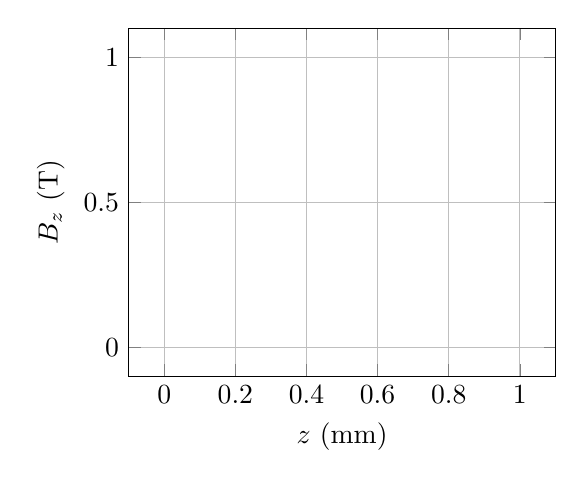
\begin{tikzpicture}
\begin{axis}[width=7cm,height=6cm,grid=major,no markers,
    xlabel={$z$ (mm)},ylabel={$B_z$ (T)}]
  \femmplot[profile=magnet-axis,component=Bz,abscissa=z,
    plot options={blue!65!black,thick}]
\end{axis}
\end{tikzpicture}
\end{codeexample}

\luafemmexampleend{axisymmetric-magnet}

\subsection{Formulation, axis regularity and boundary conventions}
The unknown is continuous piecewise-affine $A_\varphi$ on the physical
$(r,z)$ triangles, with
\[
 B_r=-\partial_z A_\varphi,\qquad
 B_z=\partial_r A_\varphi+{A_\varphi\over r},\qquad
 \mathrm dV=2\pi r\,\mathrm dr\,\mathrm dz.
\]
Axis nodes are fixed to zero automatically. Nonzero prescribed axis values
are errors. At an axis sample the regular one-sided limit is used:
$B_r=0$ and $B_z=2\partial_r A_\varphi$. Field values inside an element vary
with radius; the element's stored field is its centroid diagnostic, not a
replacement for point evaluation or volume quadrature.

Writing $\mathcal C v=(-\partial_zv,\partial_rv+v/r)$, the weak residual per
radian is
\[
 \int_\Omega r\bigl[\mathbf H\cdot\mathcal Cv-J_\varphi v\bigr]
       \,\mathrm dr\,\mathrm dz
 +\int_{\partial\Omega_w}r(cA_\varphi+g)v\,\mathrm ds=0.
\]
$\mathbf H$ includes the coercive source. A positive seven-point triangle rule
integrates the radius-weighted material residual and its consistent symmetric
Newton tangent. Regional energy uses the same quadrature. Linear tensor and
isotropic nonlinear material laws are shared with the planar solver. Spatial
coercivity directions retain the documented elementwise averaging rule.

Dirichlet data specify $A_\varphi$ in T\,m. For the counterclockwise meridional
tangent $\mathbf t=(-n_z,n_r)$, the weak Neumann/Robin convention is
\emph{$-\mathbf H\cdot\mathbf t=cA_\varphi+g$}. The sign differs from the planar
curl convention. All affine coefficients still use SI coordinates. The exact
radially weighted edge mass matrix is used. A uniform positive $B_z$ in air,
for example, requires |value=-Bz/mu0| on a natural outer vertical boundary.
An all-natural domain that touches the axis is regularity-anchored; its total
azimuthal current need not vanish.

\subsection{Exchange and validation limits}
The supported FEM input/output subset now accepts axisymmetric headers, geometry,
materials, circular winding currents and supported fixed/mixed boundaries.
ANS output writes nodal \emph{flux} $2\pi rA_\varphi$, following FEMM's convention.
FEMM uses different flux interpolation inside triangles, so its reconstructed
$B$ and $H$ from these nodal values are not an exact snapshot of our P1
$A_\varphi$ derivatives. Preserve the native cache for exact reuse, and compare
FEMM field samples under refinement. The uniform-field patch agrees to rounding;
nonuniform snapshots are subject to this interpolation difference.
The primary comparison is described in
\href{https://femm.info/doku/doku.php?id=axisymmetricformulation}{FEMM's
axisymmetric formulation note} and in the audited xfemm source.

Analytic tests cover a uniform axial field, full-revolution volume and energy,
flux orientation, natural and mixed boundary signs, a nonlinear magnet with
$H=0$, circular winding resistance and the identity $W=I\lambda/2$.
For the manufactured $A_\varphi=r^3$, $B_z=4r^2$ and
$J_\varphi=-8r/\mu_0$, radial-volume-weighted field errors at spacings
.2, .1 and .05 m are 9.287\%, 4.602\% and 2.304\%.
Analytical conductor forces check all three force methods and their signs.
The generic format matrix includes cylindrical profiles and cold/warm/shared
frozen winding caches under all three formats.

Independent axisymmetric validation compares uniform fixed/mixed fields, solenoids with air or nonlinear iron cores,
and cylindrical magnets through xfemm's native reader and independent solver. Its scope and measured errors are recorded in \nolinkurl{doc/validation.md}.
All 36 local comparisons passed; the largest peak-normalised field discrepancies
were .532\% for snapshots and 1.974\% for independent solves.
These checks establish a bounded static subset, not complete axisymmetric FEMM
parity. Kelvin exterior regions and their scaled flux pairing are described in
Section~\ref{sec:exterior}. General periodic sectors, the planar ideal model
and the circular planar open-boundary approximation remain unavailable.
The axial H model is described separately in Section~\ref{sec:currents}.
Azimuthal magnetic fields, sliding gaps and previous
solution modes remain separate work. Use domain enlargement and mesh refinement
to check exterior truncation, or use the bounded Kelvin formulation.
